\documentclass{article}
\usepackage{graphicx}
\usepackage{lscape}
\usepackage{pdflscape}
\usepackage{booktabs}

\title{Feasibility Study}
\author{Thomas Scott}
\date{1st October 2018}

\begin{document}
	\pagenumbering{gobble}
	\maketitle
	\newpage
	\pagenumbering{arabic}

	\section{Title}

	CoAP based IoT data transfer from a Raspberry Pi to Cloud 

	\section{Learning Objectives}
	
	\begin{itemize}	
	\item Use knowledge, abilities and skills for further study and for a range of employment in areas related to scientific and technical computing.
	\item Interpret legislation appropriate to computer professionals and also be aware of relevant ethical issues and the role of professional bodies.
	\item Analyse, design, and implement algorithms using a range of appropriate languages and/or methodologies.
	\item Demonstrate an understanding of the characteristics and operation of various networking technologies and communication protocols.
	\item Conduct an investigation in usage and implementation of communication protocols.
	\item Identify and make use of current scholarly research in the field.
	\item Demonstrate effective communication, decision making and creative problem solving skills, and identify appropriate practices within a professional, legal and ethical framework.
	\end{itemize}

	\section{Project Background}
	The Internet Engineering Task Force (IETF) standardized the Constrained Application Protocol ‘CoAP’ as RFC 7252 in 2014 —as a specialized web transfer protocol for constrained devices, constrained nodes and constrained networks in the Internet of Things ‘IoTs’. 
	The Constrained Application Protocol (CoAP) is a software protocol that enables simple constrained “things” such as low-power sensors and actuators to communicate interactively via the internet. 
	It runs on devices that support the User Datagram Protocol (UDP) and implements a lightweight application layer that suited for low-power, low-memory devices.

	\section{Aims}
	The aim of this project is to investigate the implementation of CoAP technology and how to use CoAP to send data to the cloud.

	\section{Objectives}
	\begin{enumerate}
	\item Explore existing research into using CoAP technology to send sensor data to a cloud service.
	\item Identify ways in which sensor data can be transferred using CoAP.
	\item Investigate and choose a cloud computing platforms to send sensor data to.
	\item Investigate the usage of CoAP over different transport layers. (UDP, TLS).
	\item Compare CoAP to similar protocols (MQTT) that data to the cloud.
	\item Implement a CoAP client on a Raspberry Pi which:
		\begin{enumerate}
			\item Connects to a sensor attached to the device
			\item Connects to the internet
			\item Can transmit data collected from the sensor to a cloud platform
		\end{enumerate}
	\end{enumerate}

	\section{Required Resources}
	\begin{itemize}
		\item Raspberry Pi 3
		\item Micro SD card
		\item Power cord
		\item Sensor DHT22
		\item Cloud Platform (To be selected as part of project)
	\end{itemize}
	
	\begin{landscape}
		
		\section{Tasks and Timescale}
		
		\begin{figure}[ht]
			\centering
			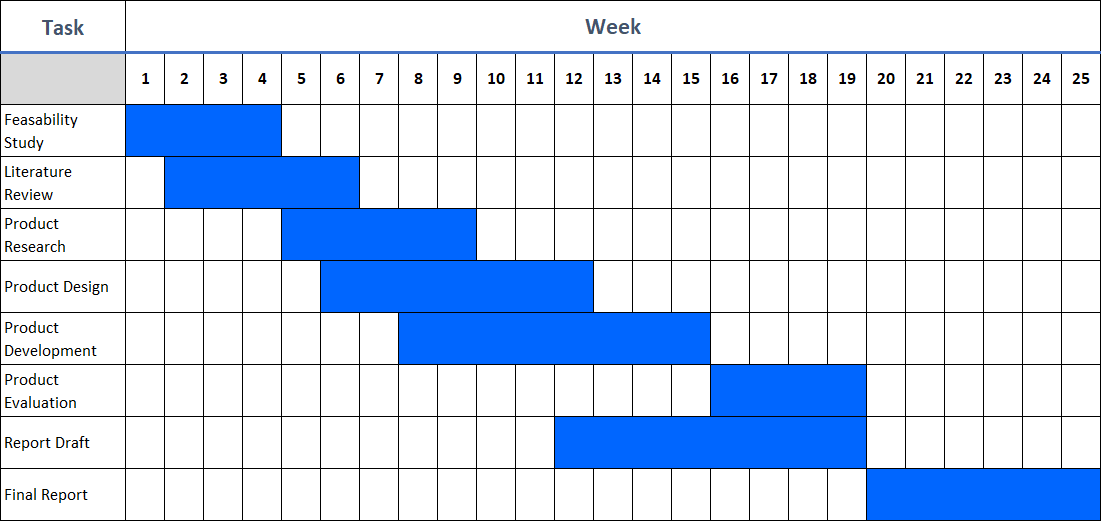
\includegraphics[width=\linewidth, height=\textheight,keepaspectratio]{gantt.png}
		\end{figure}

	\end{landscape}

	\section{Timescale dates}
	\begin{table}[h]
		\begin{tabular}{@{}llll@{}}
		\toprule
		Week & Starting & Requirement                 & Deadline      \\ \midrule
		4    & 15/10/18 & Feasibility Study submitted & 19/10/18      \\
		12   & 10/12/18 & Prototype Report uploaded   & 14/12/18      \\
		18   & 11/02/19 & Product submitted           & 22/02/19      \\
		20   & 25/02/19 & Report Outline uploaded     & 01/03/19      \\
		25   & 01/04/19 & Showcase held               & Specified day \\
		25   & 01/04/19 & Report submitted            & 05/04/19      \\ \bottomrule
		\end{tabular}
		\end{table}
		

\end{document}


